\documentclass[11pt]{article}

% Change "review" to "final" to generate the final (camera-ready) version.
\usepackage[review]{acl}

\usepackage{times}
\usepackage{latexsym}
\usepackage[T1]{fontenc}
\usepackage[utf8]{inputenc}
\usepackage{microtype}
\usepackage{graphicx}
\usepackage{amsmath}
\usepackage{amssymb}
\usepackage{booktabs}

\newcommand{\pp}[1]{#1\,\mathrm{pp}}
\newcommand{\ci}[2]{[#1, #2]}

\title{Correctness Scores Do Not Identify Safe Reasoning-Step Rollbacks: \\ A Counterfactual Study of Step Removability}

\author{Anonymous ACL submission}

\begin{document}
\maketitle

\begin{abstract}
Process reward models (PRMs) score the local correctness of reasoning steps; as chain-of-thought compression matures, correctness scores are natural candidates for deciding which steps of a generated trajectory can be pruned. We ask whether step-level correctness signals actually identify \emph{removable} steps. We introduce a counterfactual intervention protocol---control, deletion, position-and-length-matched \emph{placebo} deletion, and semantic-preserving \emph{paraphrase}---and apply it to 600 rating-balanced PRM800K steps (over 23{,}000 regenerated continuations), with replications on two further generators, a within-checkpoint thinking-mode toggle, and 300 ProcessBench steps from twelve source models. Deletion raises accuracy by $+7.2$ points on average on the rating-balanced cohort ($-0.5$\,pp when reweighted to the natural step distribution), but the gain concentrates almost entirely in steps that are both low-rated and semantically harmful ($+23.3$\,pp; phi-4: $+33.7$\,pp; external first-error steps: $+24.8$\,pp). Controls decompose the mechanism: once each placebo cutoff gets its \emph{own} control, matched innocuous deletions are inert in every group (difference-in-differences), paraphrasing the erroneous step---preserving its wrong meaning---performs like keeping it, and the anchor-group gain is target-specific through and through ($+25$\,pp): a negative anchor. Toggling the same generator into extended thinking makes the anchor vanish (anchor deletion effect $+21.8 \to -3.0$\,pp)---thinking models recover from erroneous prefixes on their own, and a long-CoT distill replicates the collapse. Crucially, no correctness signal identifies \emph{which} deletions are safe: the dataset rating ranks deletion danger below chance (AUROC $0.42$), three trained PRM checkpoints and two prompted PRM judges do no better, and step entropy is uninformative. Under deployment weighting with honest train/calibrate/test selection, certified coverage is split-unstable and certificates do not transfer---the strongest trained PRM certifies coverage that realizes $-6.3$\,pp per deletion on held-out problems---while the compression-relevant 92\% of natural traffic never certifies at tight budgets; a single probe-and-rollback generation removes all detectable excess harm (harmed-step share below its stochastic floor). Correctness scores are evidence for \emph{ranking} rollback candidates, not licenses to delete; safe pruning needs counterfactual validation. We release the audited dataset, pipeline, and benchmark.
\end{abstract}

\section{Introduction}

Process reward models assign scores to individual steps of a reasoning trajectory and have become a standard tool for verifying and steering large language model (LLM) reasoning \citep{lightman2024lets,uesato2022solving,wang2024mathshepherd}. As long chains of thought grow expensive, systems have begun pruning generated reasoning with attention-based redundancy scores \citep{choi2025think}, step entropy \citep{li2025compressing}, and likelihood-preserving token deletion \citep{singh2026llms}. Step-level \emph{correctness} scores are the obvious next candidate---PRMs are exactly the models trained to say which steps are bad---but reusing them as deletion signals embeds a silent assumption: that a step's correctness score tells us what happens to downstream reasoning if the step is \emph{removed}. Before that reuse hardens into practice, we test the assumption directly.

This assumption conflates several distinct properties of a reasoning step. A step can be locally correct yet contribute nothing that later steps use; it can be locally incorrect yet occur after the trajectory is already doomed, so removing it changes nothing; and it can be incorrect in a way that actively \emph{anchors} the continuation to a bad path, so removing it rescues the run. Whether deletion helps is a \emph{counterfactual} property of the step--generator pair, not a syntactic property of the step in isolation.

We study this gap directly. Starting from PRM800K \citep{lightman2024lets}, we sample 600 target steps balanced across human ratings ($-1/0/{+}1$), annotate each step's semantic contribution (Essential / Redundant / Harmful), and measure what actually happens when a fixed generator (Qwen3-8B; \citealp{qwen3_2025}) continues the trajectory with and without the step, four runs per condition, 2{,}400 paired outcomes. Because deleting \emph{any} step also forces the generator to re-plan---which can itself change outcomes---we additionally run a position-and-length-matched \emph{placebo} deletion for 511 of the 600 steps (1{,}514 runs), letting us decompose raw deletion effects into a target-specific component and a generic restart component. An LLM judge scores final answers; a 200-output human audit measures judge accuracy, and a full label-substitution analysis quantifies the observed effect of judge noise on every headline number ($\le 0.13$\,pp on the audited subset).

Three findings emerge. \textbf{First, correctness and contribution are correlated but far from interchangeable} (Cram\'er's $V = 0.53$; 34.5\% of steps off the expected diagonal), and deletion outcomes track the \emph{interaction}: only steps that are both low-rated and Harmful yield large reliable gains ($+23.3$\,pp), while every other rating or type group is statistically indistinguishable from zero. The pattern replicates on a second no-thinking generator from a different pretraining pipeline (phi-4: anchor effect $+33.7$\,pp) and on external ProcessBench trajectories from twelve source models; and toggling the \emph{same} Qwen3-8B checkpoint into thinking mode collapses the anchor effect ($+21.8 \to -3.0$\,pp), as does a long-CoT distill (R1-Distill-Qwen-14B; DiD semantic $-1.0$\,pp)---extended thinking itself neutralizes bad prefixes. \textbf{Second, the anchor-group gain is semantic through and through.} A single-control placebo suggests a $+10.0$\,pp generic ``restart'' component, but that contrast is confounded: half the matched cutoffs fall before the target and silently remove it. Giving every placebo cutoff its \emph{own} control (1{,}514 new runs) shows matched innocuous deletions are inert in every group, and the anchor effect is fully target-specific ($+25.4$\,pp, difference-in-differences); the paraphrase control shows it travels with meaning---rewording the erroneous step performs like keeping it, while deleting it gains $+19.2$\,pp over the paraphrase (a \emph{negative anchor}). \textbf{Third, scores are not policies.} We budget the \emph{certified net accuracy change per deleted step} (a one-sided 95\% cluster bound), which repairs a subtle flaw in transition-rate ``harm'': independent regeneration makes a null deletion on a stochastic step look 25\% harmful. Under deployment weighting with nested train/calibrate/test selection over 20 splits, correctness-based certificates are unstable (even random certifies in 9/20 splits) and do not transfer---the strongest trained PRM certifies in every split yet realizes $-6.3$\,pp per deletion on test---while the rating-$+1$ mass that compression actually targets (92\% of natural traffic) never certifies at budgets below 5\,pp. Only a trajectory-state predictor certifies coverage with reliably positive realized effect ($+8.8$\,pp per deletion). The information gap, not the intervention, is the bottleneck---and a single probe-and-rollback generation removes all detectable excess harm while raising the net gain to $+11.5$\,pp per candidate.

Our contributions: (i) a conceptual separation of step correctness, semantic contribution, and retrospective removability, with pre-specified estimands; (ii) a reusable counterfactual protocol---control / target deletion / matched placebo / semantic-preserving paraphrase---with an audited automatic evaluator; (iii) an empirical characterization of \emph{negative reasoning anchors}, replicated across two no-thinking generators and an external multi-model benchmark, and shown to vanish when the same generator thinks before answering; (iv) a signal audit spanning dataset ratings, deployed PRM scores, uncertainty, and counterfactual importance; and (v) a causal risk--coverage and rollback benchmark showing that correctness-based safety certificates do not transfer across problems, while cheap counterfactual validation removes all detectable excess harm. We release all data, code, and audits.

\section{Related Work}

\paragraph{Process supervision and PRMs.}
Step-level supervision improves credit assignment over outcome-only rewards \citep{uesato2022solving,lightman2024lets,cobbe2021training}. Math-Shepherd derives step labels from rollout success probabilities \citep{wang2024mathshepherd}; \citet{setlur2025rewarding} argue for rewarding \emph{progress} (prospective advantage) rather than local correctness; generative PRMs verify steps with explicit reasoning \citep{khalifa2025process}. Benchmarks probe what PRMs detect: ProcessBench locates first errors \citep{zheng2025processbench}, and PRMBench separates fine-grained error dimensions including redundancy \citep{song2025prmbench}. None measures what happens when a step is \emph{removed}---the counterfactual layer our protocol supplies.

\paragraph{Reasoning compression and pruning.}
Token- and step-pruning methods compress chains of thought using attention-based redundancy \citep{choi2025think}, step entropy \citep{li2025compressing}, or likelihood-preserving greedy deletion \citep{singh2026llms}; none uses PRM correctness scores as its deletion signal, which is precisely the reuse whose safety we quantify before it becomes practice. These works optimize for preserving the answer of an already-correct trajectory; we additionally quantify the \emph{repair} regime and show the two regimes respond to different signals.

\paragraph{Deletion as intervention.}
Ablation-style causal analyses of reasoning typically mask content at the token level or measure answer-probability shifts. Our design instead runs full \emph{regenerated} continuations---the deployment-relevant intervention---and controls the regeneration itself with a matched placebo, which proves essential: without it, restart effects up to $+10$\,pp would be misattributed to step semantics.

\section{Constructs and Estimands}
\label{sec:constructs}

We distinguish four properties of a step $s_t$ in trajectory $h$:
(1) \emph{local correctness}, the PRM800K rating in $\{-1,0,1\}$;
(2) \emph{semantic contribution}, whether the content of $s_t$ is needed by (Essential), irrelevant to (Redundant), or misleading for (Harmful) downstream reasoning;
(3) \emph{prospective advantage}, the change in success probability from \emph{taking} the step \citep{setlur2025rewarding};
(4) \emph{retrospective removability}, the change in success probability from \emph{deleting} the step after the fact and regenerating.
This paper measures (4) and its relation to (1) and (2).

For step $i$, let $Y^{c}_{ij}, Y^{t}_{ij} \in \{0,1\}$ be final-answer correctness under \textbf{C}ontrol (step kept) and \textbf{T}arget deletion, with $K{=}4$ independent runs per condition; matched steps (511/600) additionally receive one to four \textbf{P}lacebo runs $Y^{p}_{ij}$ (1{,}514 in total), applying the same truncation operator at a different, length-matched step $p$; every placebo run further receives an \emph{own control} $C_p$ (prefix kept through $p$; 1{,}514 runs), so the placebo can be read against its own cutoff rather than the target's, $\Delta^{\mathrm{sem,DiD}}_i = \Delta^{\mathrm{tgt}}_i - (\bar{Y}^{p}_i - \bar{Y}^{C_p}_i)$ (Section~\ref{sec:mechanism}). Pre-specified estimands (fixed in the released analysis plan before the extension cohorts ran; we did not use an external registry):
\begin{align}
\Delta^{\mathrm{tgt}}_i &= \bar{Y}^{t}_{i} - \bar{Y}^{c}_{i}, \qquad
\Delta^{\mathrm{plc}}_i = \bar{Y}^{p}_{i} - \bar{Y}^{c}_{i}, \nonumber\\
\Delta^{\mathrm{sem}}_i &= \Delta^{\mathrm{tgt}}_i - \Delta^{\mathrm{plc}}_i,
\label{eq:estimands}
\end{align}
plus run-level transition events \emph{danger} ($Y^{c}{=}1 \to Y^{t}{=}0$) and \emph{benefit} ($Y^{c}{=}0 \to Y^{t}{=}1$). Runs are independent fresh-session samples with no shared randomness across conditions; pairing control run $j$ with deletion run $j$ is a fixed bookkeeping convention whose expected transition rate equals $p^{c}_i(1-p^{t}_i)$ under any pairing, so we read danger/benefit rates as estimates of those products, not as within-seed counterfactual flips. $\Delta^{\mathrm{sem}}$ is a \emph{placebo-corrected} contrast; the paraphrase control probes its semantic reading directly (Section~\ref{sec:mechanism}). All confidence intervals are 95\% percentile intervals from a 5{,}000-replicate cluster bootstrap resampling \emph{target steps} (the unit at which interventions are applied); re-clustering by problem leaves headline intervals essentially unchanged (Table~\ref{tab:labelrobust}). Fixed seeds are released.

\section{Data and Intervention Protocol}
\label{sec:protocol}

\paragraph{Step cohort.}
From PRM800K phase-2 test trajectories \citep{lightman2024lets} over MATH problems \citep{hendrycks2021measuring} we sample 600 target steps, 200 per rating, balanced over early/middle/late positions ($201/201/198$). Semantic contribution was annotated twice, with both passes completed before any deletion outcome existed: an initial AI-assisted pass (165 Essential / 201 Redundant / 234 Harmful) and a human-calibrated re-labeling pass (198 / 199 / 203); the passes disagree on 164/600 steps (27.3\%), an explicit reliability bound (Limitations). The frozen statistical pipeline behind Tables~\ref{tab:main}--\ref{tab:placebo} uses the \emph{initial} pass as its primary label set ($-1\times$Harmful anchor: 178 steps); the calibrated pass (anchor: 160 steps, 154 shared) drives the correctness-vs-contribution crosstab below, extension-cohort sampling, and a robustness re-estimation of the anchor effects (Table~\ref{tab:labelrobust}: $+20.9$\,pp vs.\ $+23.3$\,pp---the headline survives either pass). Under the calibrated labels, rating and type are associated (Cram\'er's $V = 0.528$) with 65.5\% of steps on the expected diagonal (\,${+}1{\leftrightarrow}$Essential, $0{\leftrightarrow}$Redundant, ${-}1{\leftrightarrow}$Harmful\,)---correlated, but with a third of the cohort off-diagonal (Figure~\ref{fig:heatmap}, appendix).

\paragraph{Interventions.}
Both interventions are prefix truncations of the same trajectory: the Control prompt contains the problem plus steps $1{:}t$, the Target-deletion prompt contains steps $1{:}t{-}1$---operationally a \emph{rollback} of the most recent visible step, not an interior splice---and Qwen3-8B (temperature $0.7$, top-$p$ $0.8$) regenerates the continuation, four fresh runs per condition. The Placebo condition applies the identical truncation at a different step $p$ of the same trajectory (before or after $t$; 51\%/49\% in practice) whose token length is within $\pm 20\%$ of the target's, choosing the closest available position; 511/600 steps admit such a match (1{,}514 placebo runs), and the 89 unmatched steps differ from matched ones on no outcome-relevant covariate (max position SMD $0.298$). The steps at the placebo cutoffs are benign: none carries rating $-1$; 59\% carry rating $+1$, 11\% rating $0$, and 30\% are unrated (Table~\ref{tab:placebocomp}).

\paragraph{Outcome evaluation and audit.}
An LLM judge (Qwen3-8B, temperature 0; prompts released) marks final-answer correctness against ground truth. We audited 200 stratified outputs with human adjudication: agreement 93.5\% (F1 $0.931$), pair-transition agreement 91.7\%, and a maximum per-condition bias of $2.3$\,pp---below the pre-set gates (90\% / 5\,pp). Substituting all 200 adjudicated labels into the frozen tables moves the overall target effect by $-0.13$\,pp and the placebo-corrected effect by $-0.05$\,pp---observed sensitivity on the audited subset, not a bound on the remainder; no conclusion moves under substitution (Table~\ref{tab:judge}).

\paragraph{Replication and mechanism cohorts.}
Four extensions reuse the identical prompt protocol. (i)~\emph{Cross-generator}: 300 steps (all 100 available rating$\,-1\times$Harmful anchors, 100 rating-0, 100 rating-$1$; 103 stably-correct; positions balanced) rerun with \textbf{phi-4} (14B; a different pretraining pipeline from Qwen), 3 runs per condition, reusing the frozen matched-placebo indices; the identical 2{,}691-task list is additionally rerun with \textbf{DeepSeek-R1-Distill-Qwen-14B} (long-CoT, served locally; sampling and judge unchanged) and---holding the checkpoint fixed---with \textbf{Qwen3-8B's own thinking mode enabled} (same provider, prompts, and sampling as the primary runs).\footnote{The plan's nominal second generator (DeepSeek-R1-Distill) was unavailable via the API provider at freeze time; phi-4 matched the 7--14B budget and the no-thinking protocol (all 2{,}691 continuations parsed). The local long-CoT rerun parsed 99.0\% (raw-LaTeX JSON escapes repaired); the 28 unparseable continuations, balanced across conditions, score as incorrect.} (ii)~\emph{Semantic-preserving paraphrase} (condition C3): for a 240-step strong-control subset (80 anchors / 80 stably-correct / 80 rating-$0/1$ fragile), an independent model (Gemini 2.5 Flash) paraphrases the target step preserving its exact meaning \emph{including errors}; 221/240 paraphrases passed automatic validity checks (7.9\% excluded) and each ran 4 continuations, alongside 4 fresh matched-placebo runs (C2). (iii)~\emph{Deployed PRM scoring}: five PRMs score all 600 steps---three trained checkpoints (Qwen2.5-Math-PRM-7B, full-trajectory token-level head; Math-Shepherd's Mistral-7B PRM; RLHFlow's Llama3.1-8B PRM trained on DeepSeek rollouts) and two prompted LLM-judge PRMs (Gemini 2.5 Flash, phi-4). (iv)~\emph{External validation}: 300 ProcessBench steps \citep{zheng2025processbench} spanning GSM8K, MATH, OlympiadBench, and Omni-MATH trajectories from twelve source models (Section~\ref{sec:external}).

\section{Full-Cohort Deletion Results}
\label{sec:main}

\begin{table}[t]
\centering
\small
\begin{tabular}{@{}lrrr@{}}
\toprule
Group & Steps & $\Delta^{\mathrm{tgt}}$ (pp) & 95\% CI \\
\midrule
Overall            & 600 & $+7.21$  & $\ci{+3.88}{+10.58}$ \\
\midrule
rating $=-1$       & 200 & $+22.00$ & $\ci{+15.41}{+28.42}$ \\
rating $=0$        & 200 & $+0.25$  & $\ci{-5.41}{+5.90}$ \\
rating $=+1$       & 200 & $-0.63$  & $\ci{-5.54}{+4.21}$ \\
\midrule
Essential          & 165 & $-1.21$  & $\ci{-7.24}{+4.78}$ \\
Redundant          & 201 & $+1.12$  & $\ci{-3.87}{+6.06}$ \\
Harmful            & 234 & $+18.38$ & $\ci{+12.28}{+24.44}$ \\
\midrule
$-1\times$Harmful  & 178 & $+23.31$ & $\ci{+16.57}{+30.24}$ \\
\bottomrule
\end{tabular}
\caption{Target-deletion effects on final-answer accuracy (600 steps, 2{,}400 paired runs, cluster bootstrap over steps; initial-pass semantic labels---the calibrated-pass anchor estimate is $+20.9$\,pp, Table~\ref{tab:labelrobust}).}
\label{tab:main}
\end{table}

Deleting target steps helps on average ($+7.21$\,pp, Table~\ref{tab:main}), but the average is misleading: the entire reliable gain sits in the rating\,$=-1$ column and the Harmful row, peaking at $+23.31$\,pp for their intersection. Correct steps (rating $+1$) and Essential steps show near-zero \emph{average} effects---yet not because deletion is safe there. Danger is substantial everywhere: 15.1\% of control-correct runs flip to wrong under deletion, and even within rating\,$=-1$ the danger rate is 14.9\%. The near-zero group means arise from offsetting harm and benefit, not from inertness.

\paragraph{Trajectory state dominates raw effects.}
Stratifying by control stability makes the state-dependence explicit (Figure~\ref{fig:stability}, appendix): steps whose four control runs are all wrong gain $+33.4$\,pp from deletion (nothing to lose, 299 rescued runs), while steps whose control runs are all correct \emph{lose} $12.1$\,pp (CI $\ci{-15.5}{-8.9}$; 144 destroyed runs, zero possible gains). A deployment policy never observes these counterfactual states, which is exactly why raw deletion gains overstate what a policy can capture (Section~\ref{sec:policy}).

\paragraph{Step-level stability.}
With four paired runs per step, 377/600 steps never change outcome; 99 are strongly beneficial (gain in $\ge 3$ runs) and 57 strongly harmful. Of the 178 low-rated Harmful steps, 29\% are strongly beneficial to delete---$2.5\times$ the rate elsewhere (11\%), but far from a guarantee.

\paragraph{Cross-generator replication.}
The pattern is not a Qwen3-8B artifact. Rerunning 300 steps with phi-4 (3 runs per condition) reproduces every qualitative conclusion: overall target effect $+12.4$\,pp (CI $\ci{+8.3}{+16.8}$), anchor-group target effect $+33.7$\,pp (CI $\ci{+25.7}{+42.0}$) with own-controlled placebos inert ($-1.3$\,pp) and a DiD semantic component of $+34.9$\,pp (CI $\ci{+25.8}{+44.7}$), and rating-$0$/rating-$1$ target effects indistinguishable from zero ($+1.7$ and $+2.0$\,pp). Effect \emph{magnitudes} are generator-dependent, and step-level effect signs agree for 65\% of the 80 steps with nonzero effects under both generators---well above chance but far from deterministic.

\paragraph{Long-CoT replication.}
The same 2{,}691 tasks under DeepSeek-R1-Distill-Qwen-14B---which thinks before answering---change the picture qualitatively. Anchor-step control accuracy rises to 77.7\% (the model recovers from erroneous prefixes unaided), the overall deletion effect shrinks to $+3.4$\,pp (CI $\ci{+1.0}{+6.0}$), and the anchor-group effect of $+7.0$\,pp (CI $\ci{+2.7}{+11.7}$) is not about the anchor at all: deleting a matched \emph{innocuous} step helps just as much ($+8.0$\,pp against its own control), and the DiD semantic component is $-1.0$\,pp (CI $\ci{-7.8}{+6.3}$). Only 82/300 steps shift outcome at all: negative anchoring---and with it most of deletion's value---vanishes here, leaving only a small content-agnostic truncation benefit.

\paragraph{Thinking-mode contrast.}
The R1 replication changes model, scale, and training data at once; to isolate the mode, we rerun the same tasks on the \emph{same} Qwen3-8B checkpoint with thinking enabled (identical provider, prompts, sampling; thinking activates on every task, mean 2{,}514 reasoning tokens; 12.2\% of runs yield no parseable answer and are scored incorrect, balanced across conditions). On the anchor cell, whose no-thinking control accuracy is 26.8\% with a $+21.8$\,pp deletion effect, thinking lifts control accuracy to 83.3\% and the deletion effect drops to $-3.0$\,pp (CI $\ci{-8.0}{+2.3}$; DiD semantic $-3.5$\,pp, n.s.); only 77/300 steps shift outcome at all, and step-level effect signs agree with the no-thinking runs at chance (56\%, $n{=}32$). The collapse of negative anchoring is attributable to extended thinking itself, not to the R1 checkpoint.

\section{Mechanism: Anchors, not Restarts}
\label{sec:mechanism}

\begin{table}[t]
\centering
\scriptsize
\setlength{\tabcolsep}{1.8pt}
\begin{tabular}{@{}lrrrc@{}}
\toprule
Group & $\Delta^{\mathrm{tgt}}$ & $\Delta^{\mathrm{plc}}_{\mathrm{vs\,C}}$ & $\Delta^{\mathrm{plc}}_{\mathrm{own}}$ & $\Delta^{\mathrm{sem}}_{\mathrm{DiD}}$ (CI) \\
\midrule
Overall (511)        & $+7.97$  & $-0.57$ & $+0.46$ & $+7.52$ $\ci{+2.8}{+12.4}$ \\
rating $=-1$ (169)   & $+22.78$ & $+9.47$ & $-0.69$ & $+23.47$ $\ci{+14.4}{+32.5}$ \\
rating $=0$ (176)    & $+0.99$  & $-5.63$ & $+2.84$ & $-1.85$ $\ci{-9.7}{+6.0}$ \\
rating $=+1$ (166)   & $+0.30$  & $-5.42$ & $-0.90$ & $+1.20$ $\ci{-5.9}{+8.4}$ \\
Harmful (201)        & $+18.41$ & $+3.57$ & $-1.74$ & $+20.15$ $\ci{+12.0}{+28.4}$ \\
$-1\times$Harmful (151) & $+23.84$ & $+9.99$ & $-1.60$ & $+25.44$ $\ci{+16.1}{+34.9}$ \\
\bottomrule
\end{tabular}
\caption{Placebo decomposition (pp; initial-pass labels). $\Delta^{\mathrm{plc}}_{\mathrm{vs\,C}}$: placebo vs.\ the \emph{target's} control (frozen contrast); $\Delta^{\mathrm{plc}}_{\mathrm{own}}$: vs.\ its \emph{own} control $C_p$ (1{,}514 new runs); $\Delta^{\mathrm{sem}}_{\mathrm{DiD}} = \Delta^{\mathrm{tgt}} - \Delta^{\mathrm{plc}}_{\mathrm{own}}$. Matched innocuous deletions are inert everywhere.}
\label{tab:placebo}
\end{table}

Does deletion help because the \emph{content} of the step was harmful, or because \emph{any} deletion lets the generator restart and resample? Table~\ref{tab:placebo} answers with two placebo contrasts. Against the target's control, placebo truncation inside the low-rated groups looks strongly positive ($+9.99$\,pp)---the reading a single-control design would report as a ``restart benefit''. But this contrast confounds removing step $p$ with moving the cutoff: 51\% of matched cutoffs fall \emph{before} the target, so those placebo prefixes silently drop the erroneous step too. Splitting by side is diagnostic: cutoffs before the target yield $+21.1$\,pp against the shared control (they remove the anchor), cutoffs after it yield $-6.8$\,pp (they keep it). Giving each placebo cutoff its \emph{own} control---new $C_p$ runs that keep step $p$ and truncate after it---removes the confound: $\Delta^{\mathrm{plc}}_{\mathrm{own}}$ is null in every group ($-1.6$\,pp on anchors, $+0.5$ overall), and the difference-in-differences semantic effect \emph{rises} to $+25.4$\,pp (CI $\ci{+16.1}{+34.9}$) on anchors---essentially the entire raw effect. Deleting matched innocuous content does nothing; what matters is whether the \emph{anchor} leaves the prefix. (An identical-prompt subset bounds generation-batch drift between the frozen and new runs at $+3.1$\,pp, within noise; Table~\ref{tab:didrobust}.)

Two methodological corollaries. First, placebo deletions need their own controls: matching position and length is not enough---the single-control contrast \emph{understated} the anchor's semantic component by $\sim$12\,pp and manufactured a spurious restart component. Second, the rating-$0/{+}1$ ``semantic'' effects of the single-control analysis ($+5.7$ to $+6.6$\,pp) vanish under the difference-in-differences ($-1.9$ to $+1.2$\,pp, n.s.): target-specific removability lives \emph{only} in the anchor group.

\begin{table}[t]
\centering
\scriptsize
\setlength{\tabcolsep}{2.6pt}
\begin{tabular}{@{}lrrr@{}}
\toprule
Contrast (pp) & Anchor & Stable-corr. & Fragile-neutral \\
\midrule
C1$-$C0 (raw deletion)      & $+20.3$ & $-11.9$ & $+24.1$ \\
C1$-$C2 (vs.\ placebo)      & $\mathbf{+15.6}$ & $+16.8$ & $\mathbf{+0.0}$ \\
C3$-$C0 (paraphrase)        & $\mathbf{+1.7}$  & $-8.3$  & $+20.9$ \\
C1$-$C3 (vs.\ paraphrase)   & $\mathbf{+19.2}$ & $-2.7$  & $+4.1$ \\
C2$-$$C_p$ (placebo, own ctrl.) & $-0.7$ & $-0.8$ & $+3.9$ \\
\bottomrule
\end{tabular}
\caption{Four-condition strong controls (240 steps $\times$ 4 runs; 80 per group; paraphrase available for 221). Anchors: paraphrase $\approx$ control while deletion beats both---the \emph{content} is the anchor. Fragile-neutral: deletion, placebo, and paraphrase all match the uplift over the fragility-conditioned control (regression to the mean; the own-control row shows the operator is inert). Stably-correct: even meaning-preserving rewording hurts ($-8.3$\,pp).}
\label{tab:fourcond}
\end{table}

\paragraph{Paraphrase triangulation.}
The placebo isolates \emph{that} the target matters; a semantic-preserving paraphrase isolates \emph{why} (Table~\ref{tab:fourcond}). In the anchor group, replacing the erroneous step with an independent-model rewording that preserves its (wrong) meaning leaves accuracy at control level ($+1.7$\,pp, CI $\ci{-6.2}{+9.9}$), while deleting it gains $+19.2$\,pp over the paraphrase (CI $\ci{+8.2}{+30.1}$): the harm travels with the \emph{semantics}, not the surface form---exactly the signature the negative-anchor account predicts. The fragile-neutral group shows the mirror image: a large raw gain ($+24.1$\,pp) that placebo deletion---and even paraphrase---matches (C1$-$C2 $= 0.0$\,pp), i.e.\ nothing target-specific; the own-control row attributes the shared uplift to conditioning on fragile control runs rather than to any benefit of the operator. And stably-correct steps are harmed even by faithful rewording ($-8.3$\,pp, CI $\ci{-14.7}{-3.0}$), showing that correct reasoning chains are sensitive to perturbations that preserve meaning---deletion is not the only risky edit. A blinded 140-item human fidelity audit backs the C3 premise (97.1\% faithful or minimally deviating; zero of 46 audited anchor-group paraphrases corrected the original error), and the 19 excluded paraphrases resemble the 221 retained (Table~\ref{tab:paraexcl}).

Eight fully human-verified cases (78 audited continuations) illustrate the mechanism space---negative anchors, generic restarts, stably-correct steps destroyed by deletion---and ship with full continuations.

\section{External Validation on ProcessBench}
\label{sec:external}

Does any of this survive outside PRM800K trajectories and outside human step ratings? We sample 300 ProcessBench steps \citep{zheng2025processbench}---152 human-annotated \emph{first-error} steps and 148 \emph{locally-correct} steps, balanced across GSM8K, MATH, OlympiadBench, and Omni-MATH (75 each) and drawn from trajectories written by twelve different source models---and run the identical protocol (3 runs per condition; 204/300 steps admit a length-matched placebo; gold answers matched from source datasets for 99.5\% of records).

The core dissociation transfers. Deleting first-error steps yields $+24.8$\,pp (CI $\ci{+16.9}{+32.7}$); on the placebo-matched subset, the difference-in-differences semantic component is $+35.4$\,pp (CI $\ci{+22.8}{+48.9}$) with own-controlled placebos slightly \emph{negative} ($-8.4$\,pp)---erroneous steps in other models' reasoning are negative anchors too. Deleting locally-correct steps yields $-2.0$\,pp raw (CI $\ci{-8.3}{+4.1}$) and a $-7.1$\,pp (n.s.) semantic component: not usefully removable. One boundary emerges: the DiD semantic component is significant on GSM8K ($+37.3$\,pp) and MATH ($+21.1$\,pp) but attenuates on OlympiadBench ($+6.0$\,pp, CI crosses zero) and vanishes on Omni-MATH ($-0.6$\,pp)---and own-controlled placebos show no restart benefit there either ($+6.3$\,pp, n.s.): on problems near the generator's competence ceiling, nothing target-specific survives. Negative anchors are a phenomenon of \emph{recoverable} trajectories.

\section{Do Correctness Signals Predict Removability?}
\label{sec:signals}

If PRM-style signals suffice for pruning, they should predict the two events a policy cares about: \emph{danger} (destroying a correct run) and \emph{benefit} (rescuing a wrong one). We evaluate step-level signals with 5-fold cross-validation grouped by problem (no problem appears in both train and test), L2-regularized logistic models, and cluster-bootstrap CIs (Table~\ref{tab:predictive}, appendix).

The asymmetry matters. Signals rank \emph{benefit} moderately well: low rating and Harmful type genuinely enrich for rescuable runs. But for \emph{danger}---the safety-critical direction---the rating alone is anti-informative (AUROC $0.422$): among runs whose control is correct, low-rated steps are \emph{not} safer to delete, and conditioning on the rating actively misleads. Only features that peek at trajectory state (control stability; effectively extra compute) move danger prediction appreciably. Cheap local correctness is calibrated for ``was this step wrong?'', not for ``will removing it break the run?''.

\paragraph{Deployed PRMs, uncertainty, and counterfactual signals.}
Because ``PRM scores'' in deployment are continuous model outputs rather than dataset ratings, we scored the identical 600 steps with three trained PRM checkpoints (Qwen2.5-Math-PRM-7B, Math-Shepherd, RLHFlow-DeepSeek) and two prompted LLM-judge PRMs, plus step entropy/NLL under teacher forcing and a masked answer-probability drop $I_{\mathrm{mask}} = \log p(y^\star \mid h) - \log p(y^\star \mid h \setminus s_t)$ (Table~\ref{tab:signals}, appendix). The best trained PRM tracks the human rating almost exactly (danger AUROC $0.57$ vs.\ $0.56$), and the other two trained checkpoints sit at or below chance ($0.47$, $0.51$)---so the construct gap is not an artifact of auditing labels instead of scores. Token-level uncertainty carries no removability information at all. Two signals stand out modestly: cross-PRM disagreement (benefit AUPRC $0.34$ across the five, close behind the best single checkpoint's $0.37$), supporting uncertainty-based \emph{abstention}, and the counterfactual mask drop---informative but gold-answer-dependent, hence offline-only.

\section{From Scores to Policies: Risk--Coverage}
\label{sec:policy}

We convert the audit into a deployment question: if a system deletes the top-$k$ steps ranked by a signal, does it \emph{certifiably} not lose accuracy, and how many individual steps does it hurt? A tempting metric---the rate at which control-correct runs come back wrong after deletion---is not causal harm: outcomes are independent samples, so a null deletion on a step with $p^{c}{=}p^{t}{=}0.5$ would show $25\%$ ``harm'' from sampling disagreement alone. We therefore budget the \emph{certified net accuracy change per deleted step}: a policy is certified at budget $b$ if the one-sided 95\% lower confidence bound (problem-cluster bootstrap) of the mean $\Delta^{\mathrm{tgt}}$ over its selected steps stays above $-b$. Alongside, we report step-level \emph{tail risk}: the share of selected steps with observed $\hat\Delta_i<0$, minus the exact share expected under the null $p^{t}{=}p^{c}$ (Binomial$(4,\hat p)$ per step). Policies: random; correctness rankings (rating-first, Harmful-first, intersection-first); the three trained PRM scores; the model-D/E predictors of Section~\ref{sec:signals}; an in-sample oracle.

On the \emph{balanced} cohort this certification is degenerate: the case--control mix is so error-rich that the mean deletion effect is $+7.2$\,pp (LCB $+4.4$), and every policy---including random---certifies deleting \emph{all 600 steps} at every budget. Certification only becomes meaningful in the deployment frame, weighting steps to the natural chosen-path prevalence (next paragraph): there, deleting all traffic has LCB $-4.4$\,pp and certifies nothing below a 5\,pp budget.

\paragraph{Balanced cohort vs.\ natural prevalence.}
The cohort is case--control balanced (200 steps per rating); deployment traffic is not. Our reference frame is the annotator-chosen trajectory path of the phase-2 test split---the steps a deployed sampler would actually carry---comprising 16{,}481 rated steps: 31 rated $-1$, 1{,}224 rated $0$, 15{,}226 rated $+1$ (Table~\ref{tab:frame}). Chosen paths are error-scarce because PRM800K annotators route around bad candidates; the rated-but-rejected alternatives form a far larger error pool (26{,}256 rated completions, 23.2\% rated $-1$), and our rating-$-1$ targets are drawn from that pool and spliced onto the chosen prefix (198/200; the other rating tiers are chosen-path steps). Reweighting to the chosen-path prevalence therefore assumes spliced alternatives behave like the rare naturally-carried $-1$ steps, and adjusts rating composition only (the cohort is position-balanced by design). Under these weights the average deletion effect moves from $+7.2$\,pp to $-0.5$\,pp (CI $\ci{-5.1}{+4.0}$), with danger and benefit near parity ($9.8\%$ vs.\ $9.3\%$; Table~\ref{tab:natprev}): in natural traffic, indiscriminate deletion has no upside while the danger does not shrink. Balanced-cohort numbers are diagnostic contrasts, not deployment estimates.

\paragraph{What certifies in natural traffic.}
Under natural weights with in-sample selection (Table~\ref{tab:policy}, appendix), correctness rankings certify only the error tiers at a 1\,pp budget: rating-first covers 2.4\% of traffic ($+9.8$\,pp per deletion), Harmful-first 3.8\% ($+17.0$), and the best trained PRM score 0.02\% ($+51$). These deletions are \emph{error correction}, not compression---the rating-$+1$ mass that a pruning system actually wants to remove (92\% of traffic) never certifies at any budget below 5\,pp. The learned predictors certify 66--68\% of traffic in-sample ($+4.2$ to $+4.5$ per deletion); the oracle certifies 96\%.

\begin{table}[t]
\centering
\scriptsize
\setlength{\tabcolsep}{3.2pt}
\begin{tabular}{@{}lrrrr@{}}
\toprule
Policy & Certifies & Coverage & Net/del.\ (pp) & Tail excess \\
\midrule
Random             & 9/20  & 0.00 & $-3.7$ & 0.043 \\
rating-first       & 20/20 & 0.49 & $+0.9$ & 0.044 \\
Harmful-first      & 12/20 & 0.20 & $-1.8$ & 0.064 \\
PRM (Qwen2.5-Math) & 20/20 & 0.18 & $\mathbf{-6.3}$ & 0.089 \\
PRM (Math-Shep.)   & 19/20 & 0.33 & $+6.4$ & 0.000 \\
PRM (RLHFlow)      & 14/20 & 0.05 & $+3.3$ & 0.038 \\
Predictor (D)      & 15/20 & 0.13 & $+20.8$ & 0.000 \\
Predictor (E)      & 20/20 & 0.58 & $+8.8$ & 0.010 \\
\bottomrule
\end{tabular}
\caption{Nested policy evaluation, natural prevalence, 1\,pp budget: predictors trained on the calibration half only, coverage chosen on calibration (cluster-robust LCB), evaluated once on test; medians over 20 outer 50/50 problem splits. ``Certifies'': splits with nonzero certified coverage; ``Coverage'': median certified fraction of ranked steps; ``Net/del.'': median realized test net effect per deletion; ``Tail excess'': median harmed-step share above the stochastic floor.}
\label{tab:nested}
\end{table}

\paragraph{Honest nested selection.}
Certification must survive selection. Table~\ref{tab:nested} repeats the exercise with a full train/calibrate/test separation over 20 outer splits. Three failures emerge. \emph{Instability}: certified coverage swings from 0 to $0.9$ across splits for most policies---with $\sim$150 calibration problems, a 95\% bound is noisy enough that even \emph{random} certifies in 9 of 20 splits, realizing $-3.7$\,pp per deletion. \emph{Non-transfer}: the strongest trained PRM (danger AUROC $0.57$) certifies in every split yet realizes $\mathbf{-6.3}$\,pp per deletion on test, with the largest tail excess ($0.089$)---the certificate its calibration half grants does not describe its test half. \emph{Weak payoff}: rating-first transfers but realizes only $+0.9$\,pp per deletion at half-cohort coverage. Only the state-aware predictor E certifies in every split \emph{and} realizes a solidly positive net ($+8.8$\,pp, tail excess $0.010$). A certificate obtained on one sample of problems is not a license on the next---unless the signal actually carries removability information.

\paragraph{Rollback: one probe run buys most of the safety.}
Finally, we simulate the cheapest counterfactual validator: generate \emph{one} probe continuation after a candidate deletion, roll back unless the probe answers correctly, and evaluate on held-out runs. Applied to all 600 steps, this raises the net gain per candidate from $+7.2$\,pp (LCB $+4.4$) to $+11.5$\,pp (LCB $+9.3$) and cuts the observed harmed-step share from 12.2\% (stochastic floor 11.0\%) to 3.0\%---\emph{below} its 6.8\% floor, i.e.\ no detectable excess harm survives---at a cost of one extra generation per candidate and a 63\% acceptance rate. A do-nothing control-split shows the floor is calibrated (4.7\% observed vs.\ 3.7\% expected). Two caveats keep this honest: the probe is scored by the same gold-answer judge---an oracle relative to deployment, so the simulation upper-bounds a one-probe validator and presupposes one (e.g.\ a self-consistency vote)---and the gain is not mere extra sampling, since the same restart \emph{without} removing the target (the placebo) is inert overall ($-0.6$\,pp). Validation is not merely necessary (Sections~\ref{sec:signals}--\ref{sec:policy}); on these trajectories it is cheap relative to the value it protects.

\section{Discussion}
\label{sec:discussion}

Our results do not indict PRMs at their trained task: low ratings do flag wrong steps, and wrong steps are where deletion \emph{benefit} concentrates. The failure is direction-specific---scores carry almost no information about deletion \emph{danger}, which is governed by trajectory state and generator recoverability. Mechanistically, erroneous content behaves as an attractor for regeneration: continuations conditioned on the anchor commit to its error, while continuations from the cleaned prefix explore correct paths. The oracle--policy gap quantifies the headroom for better removability signals; Section~\ref{sec:signals} shows the obvious candidates do not close it, and the informative ones cost extra computation or gold answers. The constructive path is architectural rather than signal-side: the nominate--probe--rollback loop of Section~\ref{sec:policy} already recovers most of the oracle's safety at bounded cost.

\section{Conclusion}

Across 600 audited PRM800K steps, four generator configurations, four external datasets, and over 23{,}000 regenerated continuations, step correctness and step removability dissociate: deletion gains concentrate in low-rated \emph{Harmful} steps, part of that gain is a restart artifact that only a matched placebo can remove, the remainder travels with the step's erroneous content rather than its surface form, and no correctness signal---dataset rating, deployed PRM score, or uncertainty---ranks deletion danger usefully above chance. PRM scores are useful evidence about steps; they are not pruning policies. Systems that delete reasoning content should nominate with scores, validate counterfactually, and budget harm explicitly---and PRM benchmarks should test whether scores license the interventions built on them.

\section*{Limitations}

\textbf{Generator scope.} Primary results use Qwen3-8B without thinking; replications add phi-4, DeepSeek-R1-Distill-Qwen-14B, and a within-checkpoint thinking-mode toggle (300 steps, 3 runs each). The two no-thinking models agree qualitatively but not step-wise (anchor DiD semantics: $+25.4$ vs.\ $+34.9$\,pp; sign agreement 65\%); thinking mode on the same checkpoint neutralizes anchors, and the R1 distill replicates the collapse---so anchor-driven gains should not be assumed beyond no-thinking generation. All generators are mid-size open models on mathematical reasoning; we make no claims about frontier models or other domains. The R1-Distill replication failed at freeze time via the API provider (Section~\ref{sec:protocol}) and was completed later on local hardware; phi-4 remains the frozen second generator.
\textbf{Case--control cohort.} Rating-balanced sampling (200 per rating) supports subgroup contrasts, not deployment averages: reweighted to the natural prevalence of PRM800K phase-2 test steps ($0.2\%$ rated $-1$), the mean deletion effect is $-0.5$\,pp and anchor steps are rare. Every coverage number is a fraction of the balanced cohort (Table~\ref{tab:natprev}).
\textbf{PRM coverage.} The deployed-PRM audit covers three trained checkpoints---Qwen2.5-Math-PRM-7B, the original Math-Shepherd PRM \citep{wang2024mathshepherd}, and an RLHFlow Llama3.1-8B PRM trained on DeepSeek rollouts---plus two \emph{prompted} LLM-judge PRMs; trained \emph{generative} PRMs \citep{khalifa2025process} remain uncovered.
\textbf{Semantic label reliability.} Step types come from AI-assisted annotation with human calibration; the two label passes disagree on 27.3\% of steps. A blinded pilot (120 steps, two independent human labels each, four annotators in two pairs) reached only 61.7\% raw agreement ($\kappa = 0.40$), concentrated on the essential/redundant boundary; where annotators agreed, their consensus tracked the frozen outcomes (93\% of consensus-Harmful steps carry rating $-1$; placebo-corrected effect $+22.9$\,pp). A third annotator adjudicated all 46 disagreements, yielding final labels for all 120 pilot steps with 82\% adjudication accuracy. Type-based subgroup boundaries are therefore approximate; the headline interaction survives under either label set.
\textbf{Judge noise and self-evaluation.} The 93.5\% agreement and $\le 0.13$\,pp substitution sensitivity are measured on 200 audited Qwen3-8B outputs and do not bound error on the unaudited remainder; phi-4 and ProcessBench continuations are scored by the same judge pipeline without a fresh per-generator human audit. Because the judge and the primary generator share a checkpoint, we also regrade all 6{,}314 primary runs with a deterministic PRM800K-style normalization $+$ SymPy grader: it agrees with the LLM judge on 93.0\% of runs and reproduces the overall and anchor deletion effects within $0.9$\,pp, bounding self-evaluation bias.
\textbf{Placebo scope.} Matched placebos exist for 511/600 primary steps (position SMD $\le 0.298$); the external cohort's placebo matching uses character length ($\pm 20\%$) rather than tokenizer length, and 96/300 external steps admit no match.
\textbf{Offline policy evaluation.} Risk--coverage and rollback numbers reuse frozen runs; an online system would face distribution shift from its own deletions. The rollback probe is drawn from the same run pool it is evaluated against, which can flatter acceptance quality slightly. In-sample coverage selection flatters every policy; the nested train/calibrate/test protocol of Section~\ref{sec:policy} is the honest reading. With $K{=}4$ runs per condition, per-step harm attribution is noise-limited: the tail-risk excess over the exact stochastic floor is a conservative signal of truly harmed steps, not a per-step identification. Rollback presupposes a verifier and spends one probe generation per candidate, which must be netted against pruning savings in any deployment accounting.
\textbf{Paraphrase validity.} C3 paraphrases passed automatic meaning/length checks (7.9\% excluded), and a blinded 140-item human fidelity audit rated 97.1\% faithful or minimally deviating, with zero meaning changes among the 46 audited anchor-group paraphrases; two neutral-group paraphrases (4.3\% of that group's audited items) were judged meaning-changed. C3 conclusions rest on this audited premise.

\section*{Ethics Statement}

The study uses the public PRM800K dataset (MIT-licensed problems from MATH) and open-weight models; no personal data is processed. Beyond the authors, four annotators and one adjudicator recruited by the authors labeled reasoning steps and paraphrase fidelity for public math problems (about one hour each); they were informed of the study's purpose, and the annotation sheets collected no personal information. Deleting reasoning steps is an accuracy/efficiency intervention; our safety framing (harm budgets) is about answer correctness, not user harm. We release artifacts to support reproduction and auditing.

\bibliography{custom}

\appendix

\section{Judge Audit Detail}
\label{app:judge}

\begin{table}[h]
\centering
\small
\begin{tabular}{@{}lr@{}}
\toprule
Audited outputs & 200 \\
Binary agreement & 93.5\% \\
Correct-class F1 & 0.931 \\
Pair-transition agreement (60 pairs) & 91.7\% \\
Max condition bias & 2.3\,pp \\
$\Delta$ overall target effect after substitution & $-0.13$\,pp \\
$\Delta$ placebo-corrected effect after substitution & $-0.05$\,pp \\
\bottomrule
\end{tabular}
\caption{Judge audit summary. Gates (agreement $\ge$ 90\%, bias $\le$ 5\,pp) pass; all headline numbers are insensitive to full substitution of adjudicated labels.}
\label{tab:judge}
\end{table}

\section{Robustness and Disclosure Tables}
\label{app:robust}

\begin{figure}[h]
  \centering
  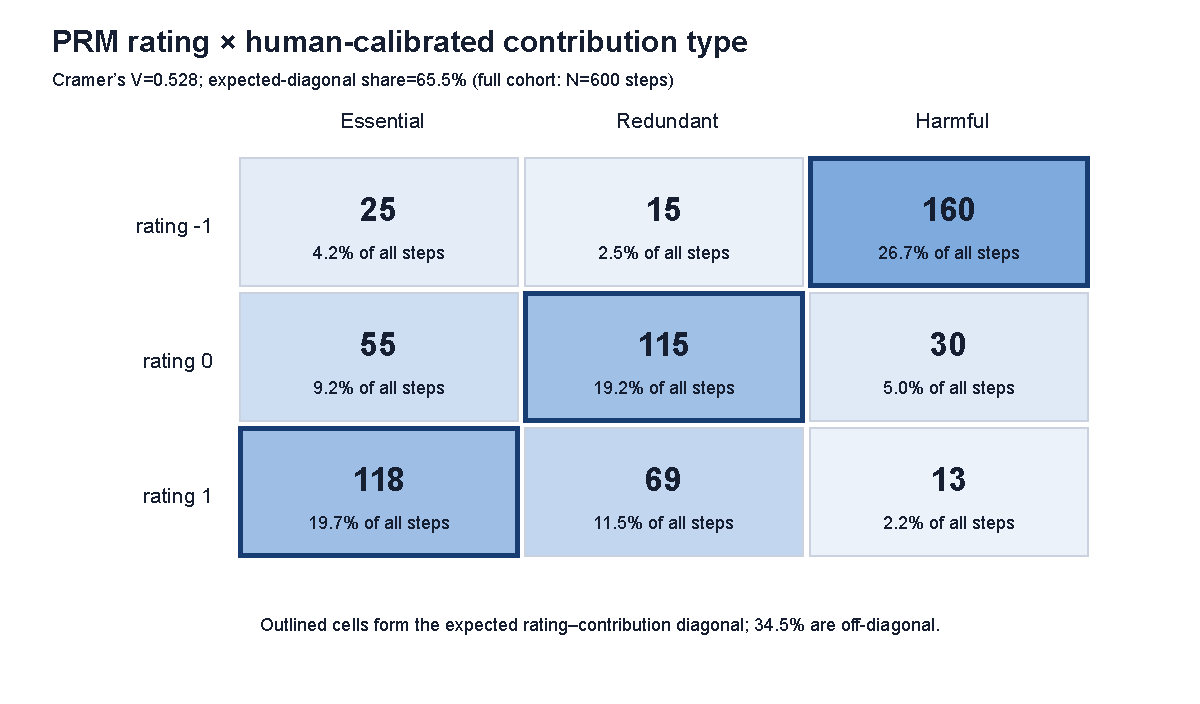
\includegraphics[width=\columnwidth]{figures/figure2_rating_step_type_heatmap.pdf}
  \caption{PRM800K rating vs.\ human-calibrated semantic contribution for the 600-step cohort. The association is strong (Cram\'er's $V=0.528$) but 34.5\% of steps are off-diagonal: local correctness does not determine contribution.}
  \label{fig:heatmap}
\end{figure}

\begin{table}[h]
\centering
\small
\setlength{\tabcolsep}{4.5pt}
\begin{tabular}{@{}lrr@{}}
\toprule
Model (features) & Danger AUPRC & Benefit AUPRC \\
\midrule
Base rate            & $0.151$ & $0.360$ \\
\midrule
A: rating only       & $0.139$ & $0.432$ \\
B: type only         & $0.208$ & $0.407$ \\
C: rating $+$ type   & $0.140$ & $0.380$ \\
D: static context    & $0.160$ & $0.412$ \\
E: $+$ trajectory state & $\mathbf{0.263}$ & $\mathbf{0.478}$ \\
\bottomrule
\end{tabular}
\caption{Out-of-fold prediction of run-level danger (base rate $15.1\%$) and benefit (base rate $36.0\%$). The rating is \emph{below chance} for danger (AUROC $0.42$, CI $\ci{0.36}{0.49}$); only trajectory-state features (model E, requiring extra runs) achieve a meaningful margin (danger AUPRC $+0.10$ over D).}
\label{tab:predictive}
\end{table}

\begin{figure}[h]
  \centering
  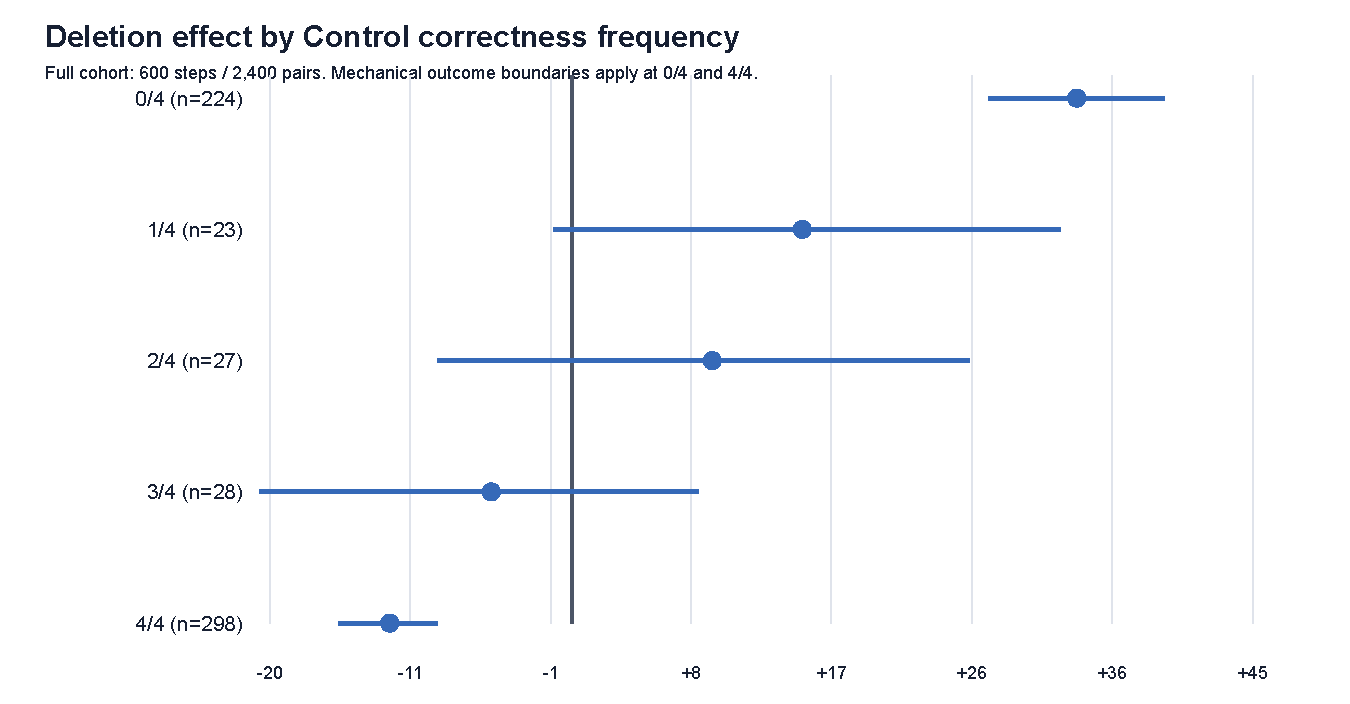
\includegraphics[width=\columnwidth]{figures/figure4_control_stability.pdf}
  \caption{Deletion effect by control-run stability. Gains exist only where control already fails; stably-correct trajectories are harmed ($-12.1$\,pp).}
  \label{fig:stability}
\end{figure}

\begin{table}[h]
\centering
\scriptsize
\setlength{\tabcolsep}{3pt}
\begin{tabular}{@{}lrrrr@{}}
\toprule
 & \multicolumn{2}{c}{Danger} & \multicolumn{2}{c}{Benefit} \\
\cmidrule(lr){2-3}\cmidrule(lr){4-5}
Signal (step-level) & AUROC & AUPRC & AUROC & AUPRC \\
\midrule
Base rate & --- & $0.15$ & --- & $0.24$ \\
PRM800K rating & $0.56$ & $0.17$ & $0.61$ & $0.34$ \\
Qwen2.5-Math-PRM-7B & $0.57$ & $0.18$ & $0.61$ & $\mathbf{0.37}$ \\
Math-Shepherd PRM (7B) & $0.47$ & $0.14$ & $0.54$ & $0.26$ \\
RLHFlow PRM (8B) & $0.51$ & $0.15$ & $0.59$ & $0.28$ \\
LLM-judge PRM (Gemini) & $0.53$ & $0.16$ & $0.51$ & $0.25$ \\
LLM-judge PRM (phi-4) & $0.49$ & $0.14$ & $0.48$ & $0.23$ \\
PRM disagreement (5 models) & $0.53$ & $0.16$ & $\mathbf{0.62}$ & $0.34$ \\
Step entropy & $0.46$ & $0.15$ & $0.48$ & $0.24$ \\
Step NLL & $0.50$ & $0.15$ & $0.49$ & $0.22$ \\
Masked answer-prob drop & $0.56$ & $0.19$ & $0.57$ & $0.30$ \\
\bottomrule
\end{tabular}
\caption{Step-level signals vs.\ deletion outcomes on the identical 600-step cohort (danger/benefit = any correct-to-wrong / wrong-to-correct transition; signals oriented so higher warns against / flags for deletion). The best benefit AUPRCs reach $0.34$--$0.37$ over a $0.24$ base---a real lift---while the best danger AUPRC ($0.19$) barely exceeds its $0.15$ base.}
\label{tab:signals}
\end{table}

\paragraph{Predictor features.} Model D uses 12 static features: indicators rating$=0$ and rating$={+}1$; indicators type$=$Redundant and type$=$Harmful (initial pass); their four interactions; position-bin indicators (middle, late); $\log(1+\text{target tokens})$; $\log(1+\text{prefix tokens})$. Model E adds the control-correct frequency (13 features). Both are L2-regularized logistic models trained with 5-fold cross-validation grouped by problem; every policy score is an out-of-fold prediction.

\paragraph{Judge configuration.} The judge is Qwen3-8B served at temperature 0, prompted with the problem, the gold answer, and the generated final answer, and instructed to return a JSON verdict on mathematical equivalence; outputs with no extractable final answer are failed by rule. The audit sampled 200 outputs stratified by condition and verdict; two annotators labeled blind to condition, with disagreements adjudicated. Full prompts, seeds, and adjudication records ship with the release.

\begin{table}[h]
\centering
\scriptsize
\setlength{\tabcolsep}{3pt}
\begin{tabular}{@{}llrrr@{}}
\toprule
Estimate & Cluster & $n$ & Effect (pp) & 95\% CI \\
\midrule
Anchor $\Delta^{\mathrm{tgt}}$, initial      & step    & 178 & $+23.31$ & $\ci{+16.6}{+29.9}$ \\
Anchor $\Delta^{\mathrm{tgt}}$, initial      & problem & 178 & $+23.31$ & $\ci{+16.2}{+30.5}$ \\
Anchor $\Delta^{\mathrm{sem}}$, initial      & step    & 151 & $+13.85$ & $\ci{+7.0}{+20.8}$ \\
Anchor $\Delta^{\mathrm{tgt}}$, calibrated   & step    & 160 & $+20.94$ & $\ci{+13.8}{+28.1}$ \\
Anchor $\Delta^{\mathrm{tgt}}$, calibrated   & problem & 160 & $+20.94$ & $\ci{+13.5}{+28.4}$ \\
Anchor $\Delta^{\mathrm{sem}}$, calibrated   & step    & 137 & $+14.84$ & $\ci{+7.5}{+22.1}$ \\
Overall $\Delta^{\mathrm{tgt}}$              & step    & 600 & $+7.21$  & $\ci{+3.9}{+10.5}$ \\
Overall $\Delta^{\mathrm{tgt}}$              & problem & 600 & $+7.21$  & $\ci{+3.7}{+10.7}$ \\
\bottomrule
\end{tabular}
\caption{Label-set and clustering robustness (fresh 5{,}000-replicate bootstraps). The anchor effect survives the calibrated label pass and problem-level clustering.}
\label{tab:labelrobust}
\end{table}

\begin{table}[h]
\centering
\small
\begin{tabular}{@{}lrr@{}}
\toprule
Rating of placebo-cutoff step & Runs & Share \\
\midrule
$+1$    & 900 & 59.4\% \\
$0$     & 167 & 11.0\% \\
unrated & 447 & 29.5\% \\
$-1$    & 0   & 0.0\% \\
\bottomrule
\end{tabular}
\caption{PRM800K ratings of the 1{,}514 placebo cutoff steps: the placebo never truncates at a known-bad step.}
\label{tab:placebocomp}
\end{table}

\begin{table}[h]
\centering
\scriptsize
\setlength{\tabcolsep}{3pt}
\begin{tabular}{@{}lrr@{}}
\toprule
 & Balanced cohort & Natural prevalence \\
\midrule
Overall $\Delta^{\mathrm{tgt}}$ (pp) & $+7.21$ $\ci{+3.9}{+10.7}$ & $-0.52$ $\ci{-5.1}{+4.0}$ \\
Run danger rate    & 8.5\%  & 9.8\% \\
Run benefit rate   & 15.7\% & 9.3\% \\
Dangerous-step share  & 15.2\% & 17.5\% \\
Beneficial-step share & 23.5\% & 17.6\% \\
\bottomrule
\end{tabular}
\caption{Balanced-cohort vs.\ natural-prevalence estimates (weights $0.2\%/7.4\%/92.4\%$ for ratings $-1/0/{+}1$, from 16{,}481 rated phase-2 test steps).}
\label{tab:natprev}
\end{table}

\begin{table}[h]
\centering
\scriptsize
\setlength{\tabcolsep}{3pt}
\begin{tabular}{@{}lrrrr@{}}
\toprule
Frame & $n_{-1}$ & $n_{0}$ & $n_{+1}$ & Total \\
\midrule
Phase-2 test, chosen path      & 31    & 1{,}224 & 15{,}226 & 16{,}481 \\
Phase-2 test, all completions  & 6{,}080 & 2{,}002 & 18{,}174 & 26{,}256 \\
\midrule
Cohort targets from chosen path  & 2   & 198 & 200 & 400 \\
Cohort targets from alternatives & 198 & 2   & 0   & 200 \\
\bottomrule
\end{tabular}
\caption{Sampling-frame audit (integer counts). The 600 cohort targets are unique steps over 303 problems; every cohort problem is in the phase-2 test split. Rating-$-1$ targets come almost entirely from rated-but-rejected alternative completions spliced onto the chosen prefix; reweighting (Table~\ref{tab:natprev}) uses the chosen-path frame.}
\label{tab:frame}
\end{table}

\begin{table}[h]
\centering
\scriptsize
\setlength{\tabcolsep}{1.6pt}
\resizebox{\columnwidth}{!}{%
\begin{tabular}{@{}lrr@{}}
\toprule
Cohort / check & $\Delta^{\mathrm{plc}}_{\mathrm{own}}$ (pp) & $\Delta^{\mathrm{sem}}_{\mathrm{DiD}}$ anch.\ (pp) \\
\midrule
Primary, anchors (151) & $-1.6$ $\ci{-6.5}{+3.2}$ & $+25.4$ $\ci{+16.1}{+34.9}$ \\
phi-4, anchors (100)   & $-1.3$ $\ci{-6.6}{+3.8}$ & $+34.9$ $\ci{+25.8}{+44.7}$ \\
M4 C2, all groups (240) & $+0.8$ $\ci{-2.7}{+4.4}$ & --- \\
Anchor cutoffs before / after & $-5.2$ / $+4.3$ & --- \\
Batch drift (128 identical prompts) & \multicolumn{2}{r}{new $-$ old $= +3.1$\,pp (n.s.)} \\
\bottomrule
\end{tabular}}
\caption{Own-control placebo (DiD) robustness. Matched innocuous deletions are inert in every cohort and group; the drift row compares fresh $C_p$ runs against frozen runs with byte-identical prompts, bounding generation-batch drift well below the contrasts of interest.}
\label{tab:didrobust}
\end{table}

\begin{table}[h]
\centering
\scriptsize
\setlength{\tabcolsep}{2.6pt}
\begin{tabular}{@{}lrrrr@{}}
\toprule
 & \multicolumn{2}{c}{Budget 1\,pp} & \multicolumn{2}{c}{Budget 3\,pp} \\
\cmidrule(lr){2-3}\cmidrule(lr){4-5}
Policy & Traffic & Net/del.\ (LCB) & Traffic & Net/del.\ (LCB) \\
\midrule
Random             & 0       & ---            & 0       & --- \\
rating-first       & 2.4\%   & $+9.8$ ($+2.0$)  & 12.2\%  & $+1.4$ ($-1.9$) \\
Harmful-first      & 3.8\%   & $+17.0$ ($+1.2$) & 3.8\%   & $+17.0$ ($+1.2$) \\
PRM (Qwen2.5-Math) & 0.02\%  & $+51.3$ ($+35.5$) & 16.3\% & $+8.2$ ($-1.8$) \\
PRM (Math-Shep.)   & 21.8\%  & $+9.6$ ($+3.0$)  & 31.3\%  & $+5.2$ ($-2.8$) \\
PRM (RLHFlow)      & 40.4\%  & $+5.0$ ($-0.6$)  & 47.7\%  & $+3.1$ ($-2.4$) \\
Predictor (D)      & 66.1\%  & $+4.2$ ($-0.8$)  & 88.9\%  & $+1.1$ ($-2.9$) \\
Predictor (E)      & 68.5\%  & $+4.5$ ($-0.1$)  & 79.7\%  & $+1.5$ ($-2.7$) \\
Oracle             & 96.4\%  & $+3.2$ ($-0.2$)  & 96.4\%  & $+3.2$ ($-0.2$) \\
\bottomrule
\end{tabular}
\caption{In-sample causal certification under natural prevalence: largest traffic coverage whose one-sided 95\% cluster LCB of net effect per deletion clears the budget, with the realized net (LCB in parentheses). In-sample $k$-selection upper-bounds every policy; the nested evaluation (Table~\ref{tab:nested}) is the honest reading.}
\label{tab:policy}
\end{table}

\begin{table}[h]
\centering
\scriptsize
\setlength{\tabcolsep}{3pt}
\begin{tabular}{@{}lrrrrr@{}}
\toprule
 & $n$ & Anchor & Stable & Neutral & Rating $-1$ \\
\midrule
Retained  & 221 & 33.0\% & 33.9\% & 33.0\% & 34.8\% \\
Excluded  & 19  & 36.8\% & 26.3\% & 36.8\% & 36.8\% \\
\bottomrule
\end{tabular}
\caption{Composition of retained vs.\ automatically excluded C3 paraphrases (mean target length: 38.0 vs.\ 32.7 tokens).}
\label{tab:paraexcl}
\end{table}

\section{Reproducibility}
\label{app:repro}

Primary numbers derive from two frozen master tables (600 steps; 6{,}314 runs) via a dependency-free Python pipeline with fixed seeds (cluster bootstrap seed 20260722, downstream 20260723); a single command regenerates every table, figure source, and the numeric manifest consumed by this paper. The extension cohorts add 17{,}126 runs (cross-generator 2{,}691; long-CoT replication 2{,}691; thinking-mode toggle 3{,}582; strong controls 1{,}843; ProcessBench 2{,}412; placebo own-controls 3{,}907 across four cohorts), each with its own checkpointed generation, judging, and analysis script under the corresponding workstream directory. Robustness artifacts (label-set re-estimation, placebo-cutoff composition, natural-prevalence reweighting, and the calibration/test policy split) are regenerated by dedicated scripts in the same release. The release includes the intervention builder, matched-placebo selector, judge-audit tooling, policy risk--coverage and rollback code, the 120-step blinded annotation pilot, PRM-scoring adapters, the M5 signal-extraction script, and the StepRem benchmark split with its evaluation script.

\end{document}
